\section{Design} \label{designsection}

\begin{figure}[htbp]
\centering
\fbox{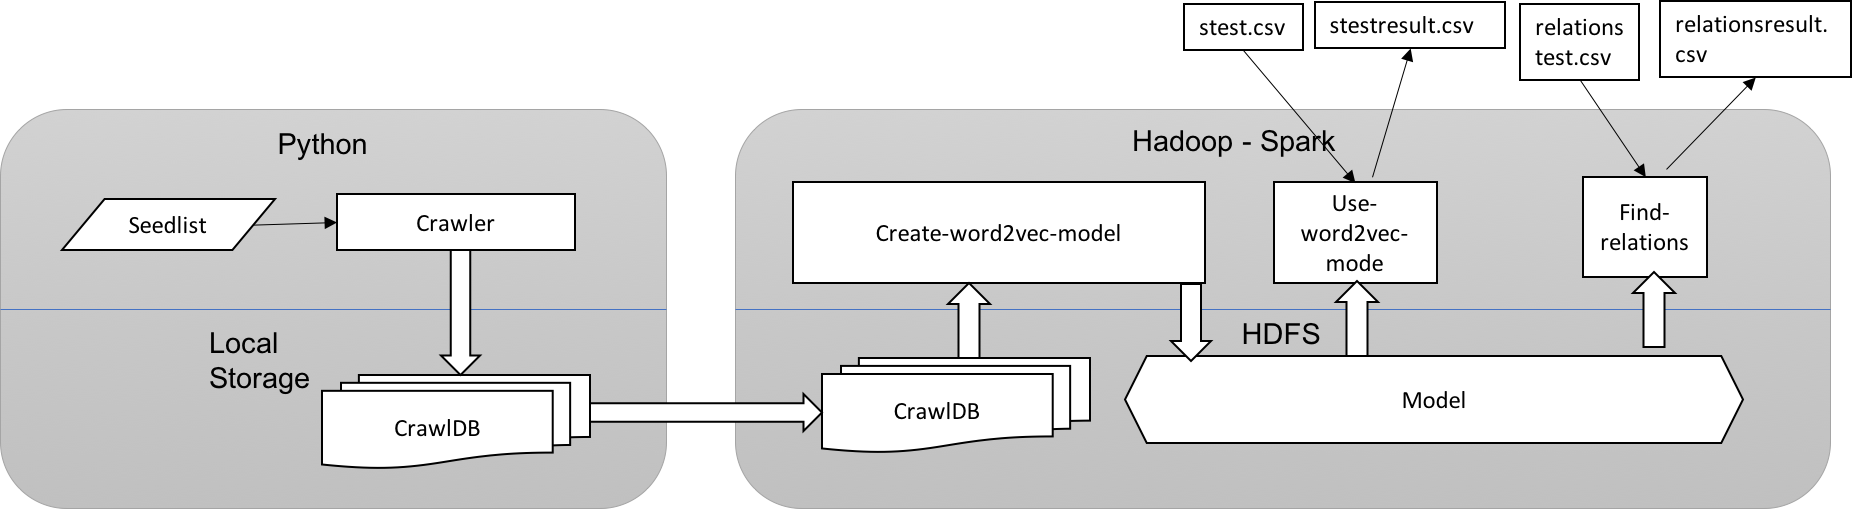
\includegraphics[width=\linewidth]{images/datapipeline.png}}
\caption{Data Pipeline.}
\label{fig:datapipeline}
\end{figure}

Figure \ref{fig:datapipeline} shows the overall data pipeline for the
project. The data pipeline has three important stages:
\begin{itemize}
\item Wiki crawler: Wiki crawler runs in batch mode on a standalone machine. It
 can download wikipedia data as explained in section \ref{wikicrawlersection}.
 Crawler creates CrawlDB which is a collection of text files. This crawler
 can be replaced or augmented with any web-crawler which can download or
 create the text files.

 \item News crawler: News crawler is responsible for downloading the news
 articles.

\item CreateWord2VecModel: This component is responsible for creating the
Word2Vec model for the text files in the CrawlDB. This model runs on spark
and stores the model on HDFS. Section \ref{createmodelsection} describes this
 component in detail.

\item UseWord2VecModel and FindRelations: These two components use the
pre-created Word2Vec model to find synonym of a word or find the relationships.
Section \ref{usemodel} describes these components in detail.
\end{itemize}

\subsection{Wiki crawler} \label{wikicrawlersection}
The Wiki Crawler component is useful to download the data from web. We
implemented
 a simple crawler using Python which can deep traverse the wikipedia pages
 and download the text from it. In our crawler implementation, a user can
 specify the seed pages from wikipedia. User can also specify the maximum
 number of pages that are required to be downloaded. The crawler first
 downloads all the pages specified in the seedlist. It then extract the links
  from each wikipedia page and puts it in a queue which is internally
  maintained by the crawler. The crawler then downloads the the linked pages.
   Since this logic is implemented in recursive manner, the crawler can
   potentially download all the wikipedia pages which can be reached from the
   pages in the seedlist.

    We followed the seedlist based crawler approach so that we can retrieve
    domain specific web pages. A well chosen seedlist can fetch large number
    of relevant web pages.

 Figure \ref{fig:crawleralgo} is the flowchart of the crawler implementation.
\begin{figure}[htbp]
\centering
\fbox{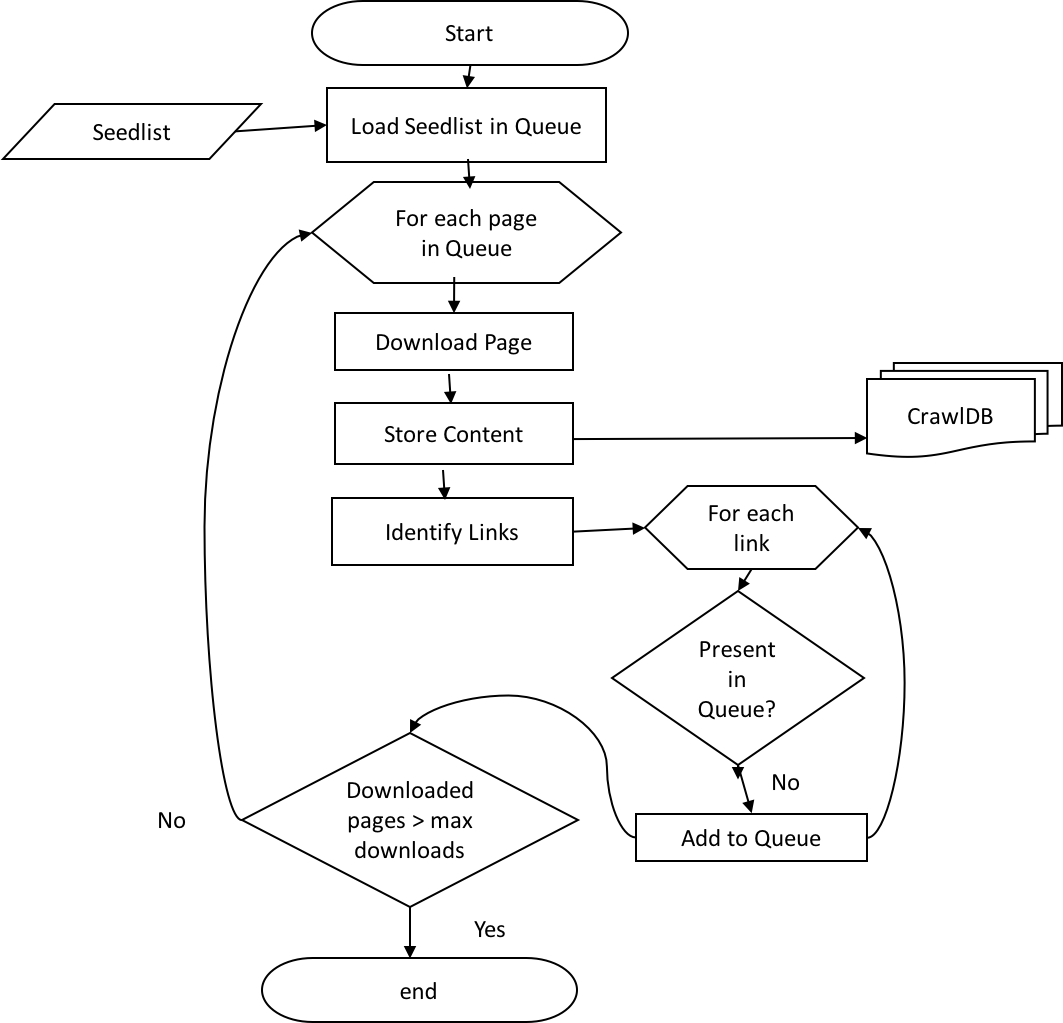
\includegraphics[width=\linewidth]{images/crawleralgo.png}}
\caption{Flowchart of crawler.}
\label{fig:crawleralgo}
\end{figure}

\subsection{News crawler} \label{newscrawlersection}
News crawler is crawler implemented in Python. It executes in
 batch mode and download latest news article related to the topics configured
 in its seedlist. The news crawler uses Google APIs
 \cite{www-google-custom-search} to search  the topics configured in the
 seedlist. Then it iterates over the result of each search, and downloads the
  original HTML page contents. The textual portion of the HTML is extracted
  using goose python library \cite{www-goose}


\subsection{Word2Vec model creation} \label{createmodelsection}
CreateWord2VecModel is Spark application implemented in Python. This
application is responsible for creating the Word2Vec model and storing it for
 later use. Figure \ref{fig:word2vecmodelflow} explains the steps involved in
  the Word2Vec model creation. We used Spark Feature Extraction
  \cite{www-sparkml-features} for implementing the steps involved in the
  Word2Vec model creation. These steps are explained below:
  \begin{itemize}
  \item Read crawled documents from HDFS
  \item For each crawled document, remove special characters from the text
  \item Tokenize text to create list of words
  \item Remove the stop words
  \item Create Word2Vec model
  \item Store the model on HDFS
  \end{itemize}

\begin{figure}[htbp]
\centering
\fbox{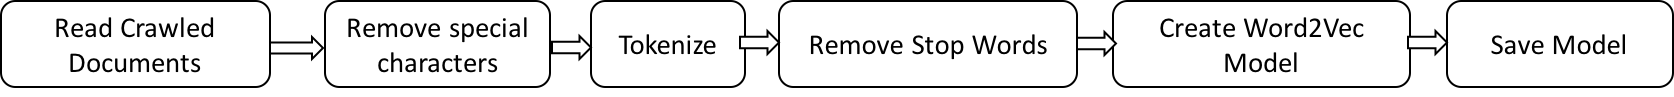
\includegraphics[width=\linewidth]{images/createword2vec.png}}
\caption{Steps involved in Word2Vec model creation.}
\label{fig:word2vecmodelflow}
\end{figure}

\subsection{Using the Word2Vec model to find synonyms and relations}
\label{usemodel}

The pre-created Word2Vec model can be queried to find the synonyms or
relations between the words. In the context of Word2Vec, synonym of the word
is the word that co-occur in similar context \cite{Goldberg2014word2vecED}.
The \textit{UseWord2VecModel} finds the synonyms for the words provided in
 the
\textit{stest.csv} file. The results are stored in \textit{sresults.csv} file.

The Word2Vec model is also used to find the relationships.
\cite{www-tensorflow} explains how the vector operations can be performed on
word vectors to derive relationships. The \textit{FindRelations} spark
application
performs the vector operations to find relationships. The relationtest.csv is
 input to the \textit{FindRelations} application. The relationtest.csv has 3
  words in
  each row. The application predicts the fourth word which has same relation to
  the thrid word as the second word related to first word. In the example below

   \textit{Sachin,Anjali,Sourav}

If \textit{Anjali} is spouse of \textit{Sachin}, then \textit{FindRelations}
application is
expected to
 predict the first name of the person who is spouse of Sourav.
  The result of \textit{FindRelations} is saved in relationsresult.csv.



